\documentclass[a4paper, 12pt]{article}
\usepackage[danish]{babel} % Language
\usepackage{minted} % Code inclusion
\usepackage{lastpage} % Pagenumbering
\usepackage{fancyhdr} % Custom header/footer
\usepackage{amsmath} % Align
\usepackage{changepage} % for the adjustwidth environment
\usepackage{multirow} % Multiple rows in tabular
\usepackage{enumitem} % space between items in list
\usepackage[page, titletoc]{appendix} % appendicies
\usepackage{wrapfig} % small figure
\usepackage[pdftitle={Programmering eksamen 2020},pdfauthor={Jens Tinggaard}, bookmarks=true]{hyperref} %References
\usepackage{cleveref} % referencing list
\usepackage[margin=1in]{geometry} %Margins
\usepackage{xcolor} % bg for minted
\usepackage{graphicx} % includegraphics
% \usepackage{attachfile} % Attach files in sources

% Biblografi
\usepackage{csquotes}
\usepackage[backend=biber, style=numeric]{biblatex}
\addbibresource{biblography.bib}
\DeclareNameAlias{default}{family-given}

\emergencystretch=1em  % hbox not too wide


\pagestyle{fancy} % Set custom page layout
\fancyhf{}% to clear existing header/footer
% Set line on header and footer width
% \renewcommand{\headrulewidth}{2pt}
% \renewcommand{\footrulewidth}{1pt}


\addto\captionsdanish{\renewcommand\appendixname{Appendiks}} % appekdiks in toc
\renewcommand{\appendixpagename}{Appendiks} %appekdiks in page


\definecolor{bg}{rgb}{0.95,0.95,0.95} % Baggrund af kode.

\newcommand{\ny}
  {
  \vskip 1em
  }

% \attachfilesetup{ % Setup af attachfile pakken.
% author={Jens Tinggaard},
% color={1 0 0},
% icon={Paperclip}
% }

% Headers and footers
\lhead{Jens Tinggaard 3.E\\ Odense Tekniske Gymnasium}
\rhead{Vejleder: JCJE\\ 1. maj 2020}

% \lfoot{\rightmark} % Subsection
\lfoot{\rightmark} % SECTION
\rfoot{Side \thepage\ af \pageref{LastPage}}


% Navn på indholdsfortegnelse
\addto\captionsdanish{\renewcommand*\contentsname{Indholdsfortegnelse}}

% Basic info
\title{Pathfinding algoritmer --- Eksamensprojekt i programmering B 2020}
\author{Jens Tinggaard (3.E)\\Odense Tekniske Gymnasium}
\date{1. maj 2020}


\setlength{\parindent}{0em} % Identeringsstørrelse = 0
% Bruges med \par

\pagenumbering{arabic}
%%%%%%%%%%%%%%%%%%%%%%%%%%%%%%%%%%%%%%%%%%%%%%%%%%%%%%%%%%%%%%%%%%%
%%%%%%%%%%%%%%%%%%%%%%%%%%%%%%%%%%%%%%%%%%%%%%%%%%%%%%%%%%%%%%%%%%%
%%%%%%%%%%%%%%%%%%%%%%%%%%%%%%%%%%%%%%%%%%%%%%%%%%%%%%%%%%%%%%%%%%%

\begin{document}

\begin{titlepage}
  \maketitle

  \begin{figure}[h]
    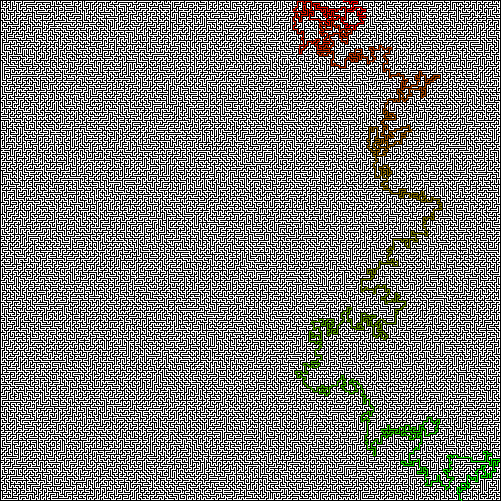
\includegraphics[width=\textwidth]{img/fp.png}
    \centering
  \end{figure}

  \thispagestyle{empty} % no page number at bottom of page
\end{titlepage}


\newpage
\tableofcontents


\newpage
\section{Indledning}
\subsection{Målsætning}
\textit{Fra projektbeskrivelsen:}\\
Jeg vil gerne lave et program, der er i stand til at illustrere en pathfinding algoritme. Jeg vil gerne vise fordelen ved en pathfinding algoritme, dette kunne f.eks. gøres ved at sammenligne med en bruteforce algoritme. Umiddelbart vil det tage udgangspunkt i labyrinter, hvor jeg vil vise hvordan de forskellige algoritmer virker.
\subsection{Krav til programmet}
\begin{itemize}
  \item Implementering af en pathfinding algoritme
  \item Kunne løse en labyrint
  \item Sammenligning med andre metoder til at løse en labyrint
  \item Visuel repræsentation af løsningen
\end{itemize}
\subsection{Udviddelser}
\begin{itemize}
  \item Visualisering af hastighed vs. størrelse af labyrint for forskellige metoder
  \item Implementering af flere algoritmer (nogle af dem fra ovenstående liste)
\end{itemize}


\newpage
\section{Om pathfinding algoritmer}\label{subsec:about}
En pathfinding algoritme er en algoritme, som bruges til at finde vej over en graf. Der findes mange forskellige algoritmer, som alle har fordele og ulemper. Et par af de mest kendte er \textit{Dijkstra}, \textit{depthfirst}, \textit{breadthfirst} og \textit{A*}. Alle disse algoritmer har til fælles, at de beskriver en fremgangsmåde, til at finde den korteste vej mellem to noder på en graf.\ny
Pathfinding er brugt til alt muligt i dag, et klassisk eksempel er navigationstjenester som Google Maps. Når brugeren har indtastet en startposition og et mål, er det nu computerens opgave at finde den korteste vej derhen. Hvis man skal fra København til Rom er der måske en idé i, at optimere algoritmen, så den ikke starter med at kigge over St. Petersborg i Rusland. Alle disse overvejelser er vigtige at gøre sig, når man skal implementere en pathfinding algoritme, da forskellige algoritmer er stærke til hver deres ting.

\subsection{Grafer, noder og kanter}
Når man snakker om pathfinding algoritmer, vil termerne \textit{graf} og \textit{node} fremkomme. Begge disse typer er abstrakte og dækker over et større område inden for datalogien. En \textit{graf} er en struktur, som indeholder et endeligt antal hjørner, også kaldet \textit{noder}. Alle disse noder har ofte nogle bestemte attributter eller egenskaber, afhængig af hvilken type graf, der er tale om. Derudover er disse noder forbundet gennem hvad der kaldes \textit{kanter} en kant er i bund og grund en forbindelse mellem to noder, man sætter ofte en vægt på kanterne (medmindre alle kanter er vægtet ligeligt). Denne vægt bruges også i beskæfigelsen med grafer --- den er meget essentiel i forbindelse med pathfinding algoritmer.\cite{graph}\ny % billede af graf: https://commons.wikimedia.org/wiki/File:Sample_Graph_for_path_finding.png
Når man har med pathfinding algoritmer at gøre, vil alle noder have følgende attributter: \textbf{Naboer} alle noder er klar over hvilke noder de ligger op ad. \textbf{Via} alle noder er klar over hvilken node der forbinder dem til startnoden. \textbf{Pris} alle noder er klar over hvor langt de har til startnoden -- målt i samlet vægt af kanter op til denne -- inden denne pris er bestemt vil den være $\infty$. \textbf{Afstand til mål} når man bruger \textit{A*}, vil alle noder også være klar over deres afstand til målnoden, denne afstand er målt direkte, såkaldt fugleflugt, hvorimod at \textit{pris} er målt i den samlede pris fra de foregående noder + vægten af kanten fra den foregående node (\textit{via}) til den nuværende.

\subsection{Prioritetskø}\label{subsec:pq}
Algoritmerne \textit{Dijkstra} og \textit{A*} gør begge brug af en prioritetskø, kaldet en \textit{priority queue} på engelsk. En prioritetskø skal ses som en liste, som er dynamisk sorteret efter et parameter. I dette tilfælde er de sorteret efter en afstand, præcis hvilken afhænger af algoritmen --- mere herom senere.

\subsection{Algoritmer}
Det vises kort, hvordan nogle af de mest kendte algoritmer virker.
\subsubsection{Depthfirst}
Depthfirst er en algoritme, som -- som navnet antager -- scanner dybden først. Betragt Node $A$, som har forbindelse til Node $B$ og $C$, algoritmen tager fat i den første af disse Noder; $B$, som i dette tilfælde har forbindelse til $D$ og $E$, igen tager algoritmen den første af disse Noder og kigger videre ud i \textit{dybden}, til slutnoden er fundet.
\subsubsection{Breadthfirst}
Breadthfirst fungerer lige modsat af depthfirst, breadthfirst kigger nemlig i bredden først. Det vil altså sige at efter Noden $B$ er undersøgt, går algoritmen videre til $C$ i stedet for $D$ som depthfirst. Bagefter kigger algoritmen på $D$ og så $E$ og derefter de Noder som er forbundet til $C$.
\subsubsection{Dijkstra}\label{subsubsec:dijk}
Dijkstra er en algoritme opkaldt efter dens skaber; \textit{Edsger W. Dijkstra}.\cite{dijkstra} Dijkstra tager fat i problemstillingen med vægting af sider på en graf, da disse spiller en rolle i udfaldet af algoritmen. Algoritmen er garenteret, til altid at finde den korteste vej fra start til slut. Algoritmen gør brug af en \nameref{subsec:pq}, som er sorteret efter afstand på alle de foregående kanter. Man tager altid fat i den lavest rangede Node i køen, hvilket vil sige at man får Noden, som er nået kortest uanset antal af foregående Noder. Man kan sige at Dijkstra er breadthfirst vægtet efter afstand i stedet for antal noder. Det betyder altså at når man har fundet en løsning, behøver man blot at markere den aktuelle kantlængde og tømme sin prioritetskø op til denne størrelse. Finder man en kortere vej, gemmes denne på samme vis. Man er på denne måde garanteret, at finde den korteste vej.
\subsubsection{A*}
A* er Dijkstra med en opgradering. Afstanden til målet regnes nemlig med, målt i fugleflugt. For hver Node gemmes den foregående Node, samt den samlede afstand stadig. Derudover gemmes afstanden til målet også (er alle Noder defineret i koordinater, kan Pythagoras bruges). Vægtningen af prioritetskøen foregår nu efter den samlede værdi af den tilbagelagte afstand, samt afstanden til målet. A* kræver altså lidt mere regnerkaft, men forbedrer samtidig målrettetheden af algoritmen, som forklaret i afsnittet "\nameref{subsec:about}".


\newpage
\section{Installation og brug}
Den letteste måde at bruge programmet på er:
\begin{minted}[fontsize=\footnotesize, bgcolor=bg]{bash}
$ git clone https://github.com/Tinggaard/pathfinding
$ cd pathfinding && virtualenv venv && . venv/bin/activate
$ pip install -e .
\end{minted}
Herefter vil det være muligt at køre hovedprogrammet (forudsat at brugeren stadig er i virtualenvironment), ved blot at kalde:
\begin{minted}[fontsize=\footnotesize, bgcolor=bg]{bash}
$ pathfinding [-h] (-i INPUT | -g width height) [-v] [-s] [-f] [-o OUTPUT]
              [-a {astar,dijkstra,breadthfirst,depthfirst,rightturn}]
\end{minted}
For at få en detaljeret beskrivelse af alle flagene, sættes flaget \texttt{-h} blot.\ny
Alternativt kan programmet installeres ved
\begin{minted}[fontsize=\footnotesize, bgcolor=bg]{bash}
$ pip install -r requirements.txt
\end{minted}
Herefter kaldes programmet som følger:
\begin{minted}[fontsize=\footnotesize, bgcolor=bg]{bash}
$ # cd pathfinding
$ ./main.py [-h] (-i INPUT | -g width height) [-v] [-s] [-f] [-o OUTPUT]
            [-a {astar,dijkstra,breadthfirst,depthfirst,rightturn}]
\end{minted}

\subsection{Eksempel}
Ønsker man at finde vej gennem \texttt{\href{https://github.com/Tinggaard/pathfinding/blob/master/mazes/perfect/1001.png}{mazes/perfect/1001.png}}, ved hjælp af breadthfirst algoritmen, samt at gemme outputtet igen som f.eks. \texttt{out/eksempel.png}, køres programmet som følger:
\begin{minted}[fontsize=\footnotesize, bgcolor=bg]{bash}
$ pathfinding -i mazes/perfect/1001.png -a breadthfirst -o out/eksempel.png
\end{minted}
% Indsæt billede!
% Indsæt billede!
% Indsæt billede!


\newpage
\section{Udarbejdning af projektet}
I forbindelse med projektet har jeg lavet et repository på GitHub (\url{https://git.io/JfINU}). Det medfølger naturligvis en README-fil, som også er vedlagt i Appendiks. Jeg vil kort gennemgå krav samt brug af programmet her, en uddybning kan findes i README-filen.

\subsection{Baggrund for projektet}
Projektet startede ud med instpiration fra denne video \cite{yt}, hvor Dr. Mike Pound, viser hvordan han har lavet et Python program, som kan finde vej gennem labyrinter. Faktisk har han også offentliggjort koden på GitHub \cite{ytgh}, hvilken jeg også har ladet mig inspirere fra.\ny
Selve pathfinding-algoritme delen af projektet er baseret på filen \texttt{\href{https://github.com/Tinggaard/pathfinding/blob/master/pathfinding/scheme.py}{pathfinding/scheme.py}}, som indeholder klasserne, mens algoritmerne ligger under \texttt{\href{https://github.com/Tinggaard/pathfinding/tree/master/pathfinding/algs}{pathfinding/algs/*}}. Filen \texttt{\href{https://github.com/Tinggaard/pathfinding/blob/master/pathfinding/main.py}{pathfinding/main.py}} er blot en wrapper til at loade filer ind i klasserne og eksekvere den gevne algoritme.
\subsection{Første udlægning}
Udover at have lavet nogle funktioner til at indlæse en labyrint enten på tekst- eller billedform, var noget af det første jeg gjorde, at lave klasser til at holde på min labyrint.
Mit første rigtige udlæg til dette (\href{https://github.com/Tinggaard/pathfinding/tree/a36e6247fe420194bf75fed42b19529c447c4c40}{a36e624}), bestod af to klasser: \texttt{Maze} og \texttt{Node}. Constructoren for \texttt{Node} klassen, så sådan ud:
\begin{minted}[fontsize=\footnotesize, bgcolor=bg, linenos]{python3}
class Node:
    def __init__(self, location: tuple):
        self.location = location # (y, x)
        self.n = None # [node_index, dist]
        self.s = None # [node_index, dist]
        self.e = None # [node_index, dist]
        self.w = None # [node_index, dist]
        self.dist_goal = np.inf
\end{minted}
Klassen har altså seks attributes, \texttt{location}, et tuple indeholdende koordinaterne til objektet og \texttt{dist\_goal}, som er afstanden til målet --- brugt i A*, samt fire naboer; \texttt{n}, \texttt{s}, \texttt{e} og \texttt{w}, som ikke har nogen værdi ind til videre, dog siger kommentaren ud for hvordan de ser ud efter at være sat --- En liste med et index på pågældende \texttt{Node}, samt afstanden til denne. Som det fremgår af linje 2, er det kun \texttt{location}, der kræves, for at lave et \texttt{Node} objekt.\\
Constructoren for \texttt{Maze}, så sådan ud:
\begin{minted}[fontsize=\footnotesize, bgcolor=bg, linenos]{python3}
class Maze:
    def __init__(self, maze: np.ndarray):
        self.maze = maze
        self.x = maze.shape[1]
        self.y = maze.shape[0]
        self.start = (0, np.argmax(maze[0]))
        self.end = (self.y-1, np.argmax(maze[-1]))
        self.nodes = self.get_nodes()
        self.node_count = len(self.nodes) # + start and end
        self.gen_graph()
\end{minted}
Klassen tager altså ét argument, til sin constructor, ud fra hvilken hele klassen dannes. Dette argument er et binært 2D numpy array\cite{ndarray}, som udelukkende består af 1- og 0-taller, hvor 1 fortolkes som sti, mens 0 er væg. Startnodens placering SKAL være i toppen af labyrinten, mens slutnoden på lige vis SKAL være i bunden af labyrinten, ellers fungerer programmet ikke! Linje 6 og 7 finder koordinaterne for hhv. start og slutnoden, ved at kalde funktionen \texttt{np.argmax(maze[i])}, som finder indexet, på den største værdi af input arrayet.\cite{argmax} På linje 8 kaldes \texttt{self.get\_nodes()} metoden, som finder alle noder i \texttt{self.maze}, ved simpelthen blot at se om den pågældende pixel, for det første er hvid (1), samt den ligger i et kryds mellem andre hvide pixels. Se den fulde funktion \href{https://github.com/Tinggaard/pathfinding/blob/a36e6247fe420194bf75fed42b19529c447c4c40/src/scheme.py\#L42-L70}{her}.
\subsection{Implementering af algoritmer}
Den første algoritme jeg implementerede, er faktisk ikke en af de ovennævnte, men i stedet en "højresvingsmetode", som blot drejer til højre ved hvert kryds og på den måde altid følger den sammve væg. Det er en klassisk taktik, hvis man ikke kan se hele labyrinten, f.eks. som menneske inde i en. Metoden blev implementeret under commit \texttt{\href{https://github.com/Tinggaard/pathfinding/commit/ea5096e2b794b00aa5d763989cb4e1e20371a383}{ea5096e}}. Det er dog ikke den algoritme jeg vil gennemgå her, men i stedet Dijkstra, som blev implementeret ved commit \texttt{\href{https://github.com/Tinggaard/pathfinding/commit/cd33a780b68f2ce17c7fac8a2f9f56d4f25ec44d}{cd33a78}}.\ny
Som det kort blev gennemgået i afsnittet "\nameref{subsubsec:dijk}", virker Dijkstra ved brug af en prioritetskø, som holder styr på den tilbagelagte længde, for hver Node og at algoritmen altid arbejder med den Node, som har tilbagelagt kortest afstand.\\
Nedenstående kode, viser et kort udtræk (linje 27-58) af filen \texttt{\href{https://github.com/Tinggaard/pathfinding/blob/cd33a780b68f2ce17c7fac8a2f9f56d4f25ec44d/src/algs/dijkstra.py\#L27-L58}{pathfinding/algs/dijkstra.py}}, som den så ud ved pågældende commit (tomme linjer og kommentarer fjernet).
\begin{minted}[fontsize=\footnotesize, bgcolor=bg, linenos]{python3}
while pq:
    current = hq.heappop(pq)
    if current.dist > goal:
        break
    if current == end:
        goal = current.dist
    for near in current.nearby:
        if near is not None:
            node = self.get_node(near)
            if not visited[node.location]:
                visited[node.location] = True
                cy, cx = current.location
                ny, nx = node.location
                distance = abs(cy-ny) if cy-ny != 0 else abs(cx-ny)
                node.dist = current.dist + distance
                node.via = self.get_node_index(cy, cx)
                hq.heappush(pq, node)
\end{minted}
\textit{Forud for denne kode, bliver der erklæret nogle variabler, som bruges i løbet af loopet.} I linje 1, sættes et loop til at køre, så længe der stadig er indhold i listen \texttt{pq}, da en liste evalueres til at være \textit{sand}, hvis den indeholder noget, ellers er den \textit{falsk} i hvilket tilfælde loopet stopper. Variablen \texttt{current} bliver sat til det første index af prioritetskøen (modulet \texttt{heapq}\cite{heapq} er importeret som \texttt{hq}), som er en instance af \texttt{Node} klassen, de bliver sorteret, da \texttt{\_\_lt\_\_()} metoden er erklæret for klassen, som kan sammenligne \texttt{self.dist} mellem to \texttt{Node} objekter, tak til \cite{so:hqsort}.
Line 3-4 fortæller loopet at stopper, hvis \texttt{current}s distance er lig med \texttt{goal} (initialiseret til $\infty$). Linje 5-6 sætter \texttt{goal} til at være lig \texttt{current}s distance, hvis den aktuelle node er identisk med slutnoden. På linje 7 initialiseres et for-loop, som itererer over alle nabonoderne for den aktuelle node. Linje 8 tjekker om naboen er en node (ikke blot en mur) og sætter så \texttt{node} til at være lig nabonoden vha. metoden \texttt{\href{https://github.com/Tinggaard/pathfinding/blob/cd33a780b68f2ce17c7fac8a2f9f56d4f25ec44d/src/scheme.py\#L121-L122}{get\_node()}}, som returnerer en \texttt{Node}, baseret på et index i \texttt{self.nodes}. Inden while-loopet har jeg også lavet et array af samme størrelse som \texttt{self.maze}, bestående af boolske udtryk, på om det enkelte felt har været besøgt før (alle felter initialiseret til \texttt{False}). På linje 10 tjekker jeg så om det aktuelle nabofelt har været besøgt førhen, ellers sættes feltet til at være besøgt på linje 11. Afstanden mellem den aktuelle node og nabonoden findes på linje 12-14 og nabonodens afstand sættes til at være denne + den tidligere afstand til \texttt{current} på linje 15. Linje 16 sætter nabonodens \texttt{via} til at være koordinaterne for \texttt{current} og slutteligt lægges nabonoden ind i prioritetskøen på linje 17.\ny
Dette er blot en kort gennemgang af hvordan jeg har implementeret Dijkstra, den endelige version af koden har lidt småændringer hist og her, men konceptet er det samme. Det med at have et boolsk array er dog lidt specielt og kan kun tillades, da kanternes vægt er lig med den faktiske afstand. Ellers kunne der være en smutvej mellem to noder, som blot blev sprunget over, hvorved den korteste afstand faktisk ikke blev fundet.

\newpage
\section{Konklusion}


\newpage
\setlength\bibitemsep{10pt}
\printbibliography[
heading=bibintoc, %Er med i indholdsfortegnelsen
title={Litteratur}, %Titel
]


\newpage
\begin{appendices}
\end{appendices}

\end{document}
